\begin{table*}[t]
\small
\caption{Performance Comparison.}
\Description[The table reports the performance of all models on all four datasets]{The table reports the Recall@5, Recall@10, NDCG@5, NDCG@10 performance of all models on all datasets. It also shows the relative improvement of our model compared to the strongest baselines. Of all the models BERT is usually the strongest baseline. MEANTIME always performs better than any other baseline.}
\label{tab:results}
\begin{tabular}{@{}llrrrrrr@{}}
\toprule
Datasets & Metrics   & MARANK & SAS    & TISAS        & BERT         & MEANTIME        & Improvement \\ \midrule
ML-1M    & Recall@5  & 0.4427 & 0.5708 & \underline{0.5869} & 0.5862       & \textbf{0.6415} & 9.31\%      \\
         & Recall@10 & 0.5993 & 0.6966 & \underline{0.7102} & 0.6987       & \textbf{0.7412} & 4.36\%      \\
         & NDCG@5    & 0.3042 & 0.4142 & 0.4307       & \underline{0.4420} & \textbf{0.4932} & 11.58\%     \\
         & NDCG@10   & 0.3548 & 0.4550 & 0.4708       & \underline{0.4786} & \textbf{0.5255} & 9.81\%      \\
ML-20M   & Recall@5  & 0.3938 & 0.5274 & 0.5412       & \underline{0.5910} & \textbf{0.6225} & 5.34\%      \\
         & Recall@10 & 0.5503 & 0.6887 & 0.7021       & \underline{0.7176} & \textbf{0.7491} & 4.39\%      \\
         & NDCG@5    & 0.2665 & 0.3700 & 0.3814       & \underline{0.4469} & \textbf{0.4739} & 6.04\%      \\
         & NDCG@10   & 0.3170 & 0.4223 & 0.4336       & \underline{0.4879} & \textbf{0.5150} & 5.55\%      \\
Beauty   & Recall@5  & 0.1577 & 0.2011 & 0.2081       & \underline{0.2271} & \textbf{0.2470} & 8.78\%      \\
         & Recall@10 & 0.2302 & 0.2714 & 0.2805       & \underline{0.3095} & \textbf{0.3330} & 7.58\%      \\
         & NDCG@5    & 0.1085 & 0.1464 & 0.1512       & \underline{0.1633} & \textbf{0.1764} & 8.05\%      \\
         & NDCG@10   & 0.1318 & 0.1689 & 0.1745       & \underline{0.1898} & \textbf{0.2041} & 7.52\%      \\
Game     & Recall@5  & 0.2846 & 0.3925 & 0.3857       & \underline{0.4211} & \textbf{0.4752} & 12.85\%     \\
         & Recall@10 & 0.4217 & 0.5201 & 0.5085       & \underline{0.5590} & \textbf{0.6100} & 9.12\%      \\
         & NDCG@5    & 0.1893 & 0.2735 & 0.2735       & \underline{0.2970} & \textbf{0.3446} & 16.03\%     \\
         & NDCG@10   & 0.2334 & 0.3147 & 0.3133       & \underline{0.3415} & \textbf{0.3882} & 13.67\%     \\ \bottomrule
\end{tabular}
\end{table*}

\subsection{Setup}
\subsubsection{Datasets}
We evaluate our model on four real-word datasets with various domains and sparsity: MovieLens 1M~\cite{movielens}, MovieLens 20M~\cite{movielens}, Amazon Beauty~\cite{amazondataset} and Amazon Game~\cite{amazondataset}. We follow the common data preprocessing procedure from~\cite{TRANSREC, SASRec, TISASRec, BERT4Rec}. We convert each dataset into an implicit dataset by treating each numerical rating or review as a presence of a user-item interaction. We group the interactions by user ids and then sort them by timestamps to form a sequence for each user. Following the custom practice~\cite{TRANSREC, SASRec, TISASRec, BERT4Rec},  we discard users and items with less than five interactions to ensure the quality of the dataset.

% We evaluate our model on four real-world datasets with various domains and sparsity. We provide their statistics next to their names as <the number of users, the number of items, the number of interactions>.
% \begin{itemize}

% \item {\textbf{MovieLens 1m} <6K, 3.4K, 1M>} %<6040, 3416, 1 M>}
% %\footnote{http://files.grouplens.org/datasets/movielens/ml-1m.zip}
% : A popular and traditional benchmark dataset from MovieLens~\cite{movielens}.

% \item {\textbf{MovieLens 20m} <138K, 18K, 20M>}% <138493, 18345, 20 M>}
% %\footnote{http://files.grouplens.org/datasets/movielens/ml-20m.zip}
% : A larger dataset from MovieLens~\cite{movielens}. 

% \item {\textbf{Amazon Beauty} <40K, 55K, 0.35M>} %<40226, 54542, 0.35 M>}
% %\footnote{http://snap.stanford.edu/data/amazon/productGraph/categoryFiles/ratings\_Beauty.csv}
% : Product reviews from Amazon~\cite{amazondataset} where the top category is "Beauty".

% \item {\textbf{Amazon Game} <29K, 23K, 0.28M>} %<29341, 23464, 0.28 M>}
% %\footnote{http://snap.stanford.edu/data/amazon/productGraph/categoryFiles/ratings\_Video\_Games.csv}
% : Product reviews from Amazon~\cite{amazondataset} where the top category is "Game".
% \end{itemize}

% We follow the common data preprocessing procedure from~\cite{TRANSREC, SASRec, TISASRec, BERT4Rec}. We convert each dataset into an implicit dataset by treating each numerical rating or review as a presence of a user-item interaction. We group the interactions by user ids and then sort them by timestamps to form a sequence for each user. Following the custom practice~\cite{TRANSREC, SASRec, TISASRec, BERT4Rec}, we discard users and items with less than five interactions to ensure the quality of the dataset. % The statistics of the processed datasets are summarized in Table-\ref{tab:datastats}.

%\begin{table}
%    \caption{Statistics of datasets.}
%    \label{tab:datastats}
%    \begin{tabular}{@{}lllrll@{}}
%    \toprule
%    Datasets & \#Users & \#Items & \#Actions & Density & Span(Days) \\ \midrule
%    ML-1m    & 6040    & 3416    & 1M   & 4.84\% & 1040 \\
%    ML-20m   & 138493  & 18345   & 20M  & 0.79\% & 7387 \\
%    Beauty   & 40226   & 54542   & 0.35M & 0.02\% & 4965 \\
%    Game     & 29341   & 23464   & 0.28M & 0.04\% & 5510 \\
%    \bottomrule
%    \end{tabular}
%\end{table}

\subsubsection{Evaluation}
To evaluate the performance of each model, we adopt the widely used \textit{leave-one-out} evaluation task. For each user's item sequence, we hold out the last item for test, and the second last item for validation. We use the rest for training. We follow the common practice~\cite{SASRec, TISASRec, BERT4Rec} of letting the model rank the ground truth item together with 100 randomly sampled negative items which haven't yet been interacted by the user. As in~\cite{BERT4Rec}, we sample the negative items according to their popularity to make the task more realistic.
To score the ranked list, we use two common metrics: \textit{Recall}, and \textit{Normalized Discounted Cumulative Gain} (NDCG). Both Recall@K and NDCG@K are designed to have larger values when the ground truth item is ranked higher up in the top-k list. We report with $K=5\text{ and }10$.


\subsection{Baselines Models \& Implementation Details}
%To validate the effectiveness of our method, we compared its performance with the following baseline models:
%\begin{itemize}
%\item {\textbf{MARank}}~\cite{MARANK}: A model that applies multi-order attention to the user's most recently interacted items to capture their individual and union-level dependencies.
%\item {\textbf{SASRec}}~\cite{SASRec}: One of the earlier models that applies uni-directional self-attention mechanism to capture the dynamic item dependencies in the user's item sequence.
%\item {\textbf{TiSASRec}}~\cite{TISASRec}: A model that improves the performance of SASRec~\cite{SASRec} by inserting the time interval information between items into attention operation.
%\item {\textbf{BERT4Rec}}~\cite{BERT4Rec}: A model that applies bi-directional transformer architecture (BERT~\cite{BERT}) and Cloze task to improve the sequential prediction capability.
%\end{itemize}
%We omitted some of the older models (e.g. BPR~\cite{BPR}, NCF~\cite{NCF}, FPMC~\cite{rendle2010factorizing}, TransRec~\cite{TRANSREC}, GRU4Rec+~\cite{hidasi2018recurrent}, CASER~\cite{CASER}, ...) that have already been outperformed by the models presented here. For all baseline models, we translated the code \footnote{https://github.com/voladorlu/MARank} \footnote{https://github.com/kang205/SASRec} 
%\footnote{https://github.com/JiachengLi1995/TiSASRec}
%\footnote{https://github.com/FeiSun/BERT4Rec}
%provided by the corresponding authors into \verb|PyTorch| to ensure a coherent comparison under the same framework. 
In order to validate the effectiveness of our method, we compare it with the state-of-the-art baselines: MARank~\cite{MARANK}, SASRec~\cite{SASRec}, TiSASRec~\cite{TISASRec}, and BERT4Rec~\cite{BERT4Rec}. These models are evaluated based on the code provided by the authors.
%We performed an extensive grid-search over the hyperparameters to ensure fairness.
We implemented MEANTIME\footnote{Our code is available at https://github.com/SungMinCho/MEANTIME} with \verb|PyTorch|.
%We report the optimal result for each baseline
%hidden dimension size $h \in \{16, 32, 64, 128\}$, head number $n \in \{2, 4\}$, dropout ratio $\in \{0.2, 0.5\}$, and weight decay $wd \in \{0, 0.00001\}$. For TiSASRec, we also performed a grid-search over the max time intervals $\in \{256, 512, 2048\}$, including the authors' suggestions. Other settings such as parameter initialization or model-specific parameters followed the suggestions of the authors. We report the optimal result for each baseline.
All models are fully tuned through an extensive grid-search on hyperparameters: hidden dimension $h \in \{16, 32, 64, 128\}$, number of heads $n \in \{2, 4\}$, dropout ratio $\in \{0.2, 0.5\}$, and weight decay $wd \in \{0, 0.00001\}$. We used the same maximum sequence length ($N=200$ for MovieLens, $N=50$ for Amazon) and the number of layers ($L = 2$) for all transformer-based models to ensure fairness. We train all models until their validation accuracy doesn't improve for 20 epochs, and then report with the test set. We report the optimal result for each model.
%All models are optimized with Adam with learning rate of 0.001, and batch size of 256. We clip the gradients whose $l_2$ norm is greater than 5.
%Since all self-attention models (SASRec, TiSASRec, BERT4Rec, MEANTIME) share a somewhat similar architecture, we use the same number of layers $L = 2$, heads $n = 2$, and 
%We used mask probability $\rho = 0.2$ for ML-1M and ML-20M, and $\rho = 0.6$ for Amazon Beauty and Game, for both BERT4Rec and MEANTIME. 
%Other parameters for MEANTIME were chosen empirically: $h = 128$ and $wd = 0$ for ML-1M and ML-20M, $h=16$ and $wd = 0.00001$ for Amazon Beauty, $h=64$ and $wd = 0.00001$ for Amazon Game, and dropout ratio $= 0.2$, $freq = 10^4$, $\tau = 1$ for all datasets. We use all 6 block types for experimentation. We train all models until their validation performance doesn't improve for 20 epochs, and then report with the test set.
%Other parameters for MEANTIME were chosen empirically: $h = 128$ for ML-1M and ML-20M, $h=32$ for Amazon Beauty, $h=64$ for Amazon Game, and dropout ratio $= 0.2$, $freq = 10^4$,\text{ and } $\tau = 1$ for all datasets.
%We use all 6 block types for experimentation.
As for embedding types in MEANTIME, we used the best combination of embedding types among all possible combinations with $n=2, 4$: \textbf{Day+Pos+Sin+Log} for MovieLens 1M and 20M, \textbf{Day+Sin+Exp+Log} for Amazon Beauty, and \textbf{Day+Pos+Sin+Exp} for Amazon Game. 


\subsection{Results}
Table \ref{tab:results} shows the performance of all models on four datasets. It also shows the relative improvements of our model compared to the strongest baselines.
% Among the baselines, MARank performs the worst, presumably because it only looks at the most recent items of the user. TiSASRec outperforms SASRec, due to its usage of time intervals which makes its attention operation more comprehensive. As reported in \cite{BERT4Rec}, BERT4Rec outperforms SASRec due to its use of bi-directional transformers (as opposed to uni-directional transformers), which gives stronger prediction capabilities. BERT4Rec even outperforms TiSASRec in almost all cases. This is interesting considering that BERT4Rec does not utilize time interval information at all.
Our model gives the best performance in all metrics and datasets. On average, MEANTIME achieves \textbf{9.07\%}, \textbf{6.36\%}, \textbf{10.43\%}, and \textbf{9.14\%} improvements over the strongest baselines in Recall@5, Recall@10, NDCG@5 and NDCG@10, respectively. Given that we tune all models under the same set of hyperparameters (including the number of attention heads), we can deduce that the performance boost comes from the novel multi-temporal embeddings and attention operations that we proposed. Especially, although TiSASRec uses additional temporal information, it does not show impressive improvement over SASRec and BERT4Rec. We argue that using a single embedding scheme throughout all attention heads was a hindrance to their potential improvement. In contrast, each attention head takes different temporal embedding to extract specialized patterns in our design. This joint design of diverse temporal embeddings and attention mechanism was the key to our improvement.


\subsection{Effect of Multi-temporal Embeddings}
\begin{figure*}[t]
  \centering
  \begin{minipage}[t]{.49\linewidth}
    \centering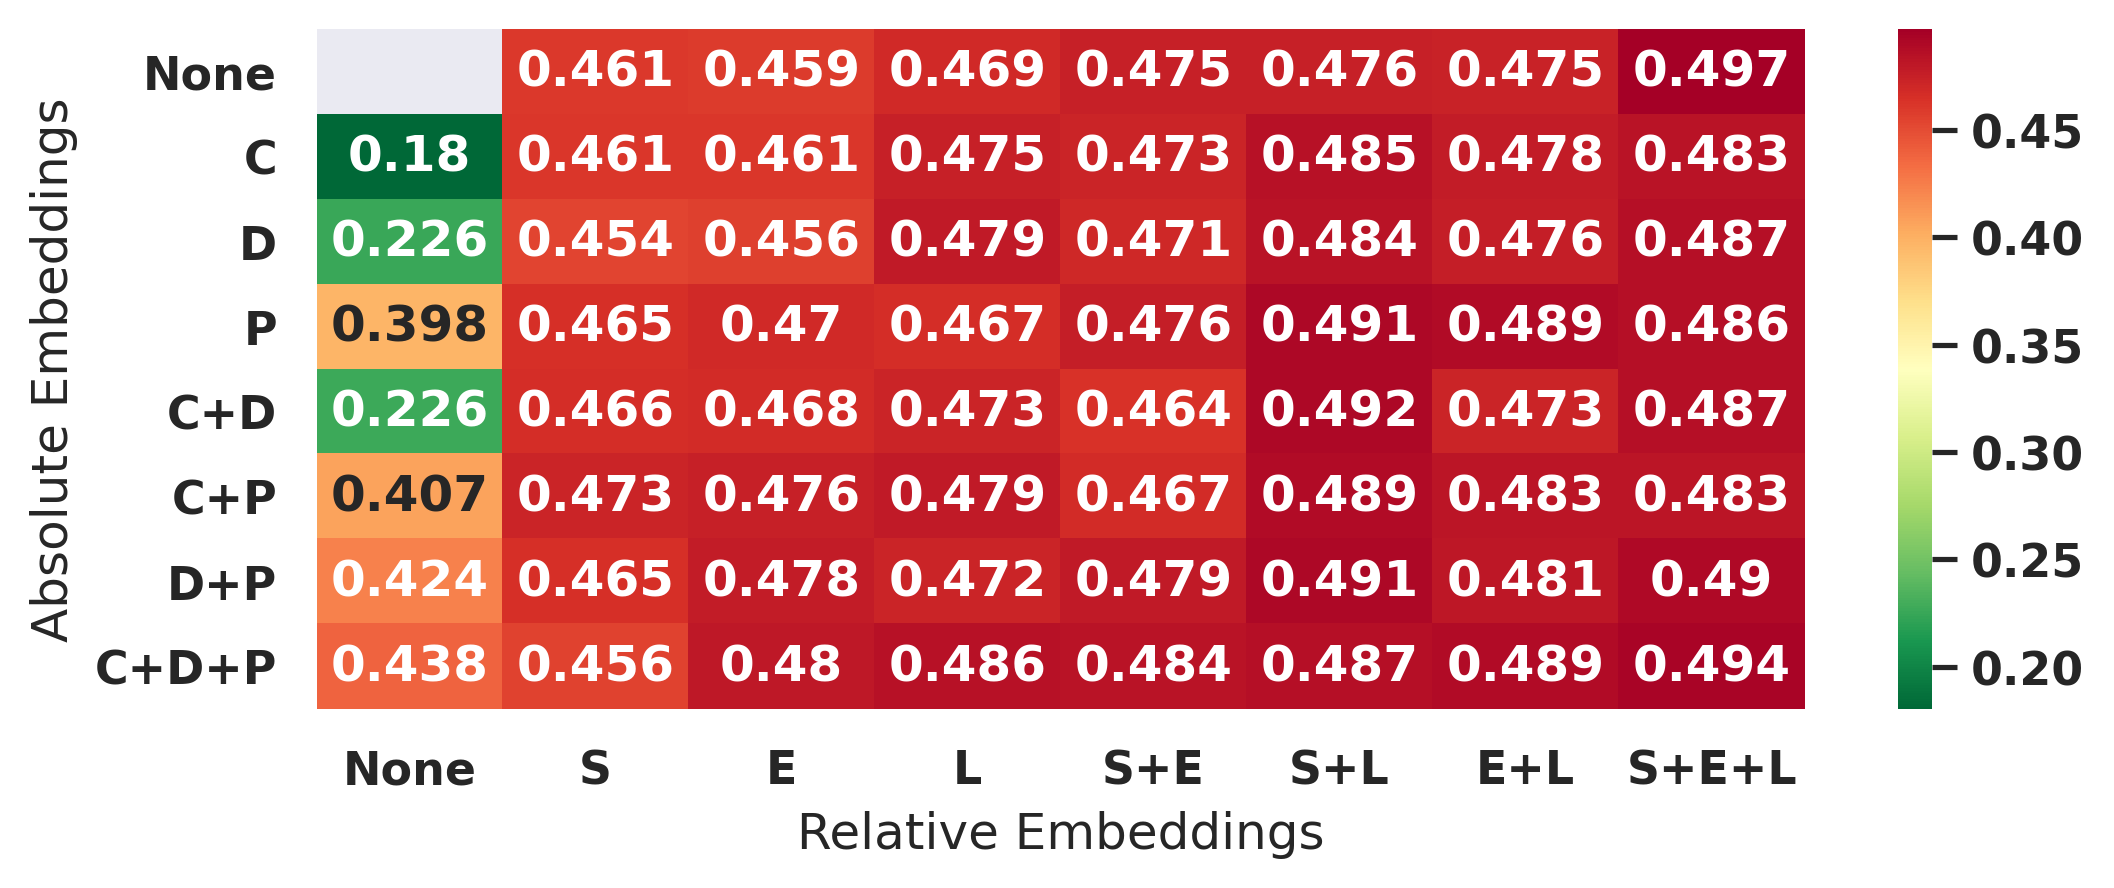
\includegraphics[width=\linewidth]{figures/combinations/ml-1m_60.png}
    %\caption{MovieLens 1M}
  \end{minipage}
  \begin{minipage}[t]{.49\linewidth}
    \centering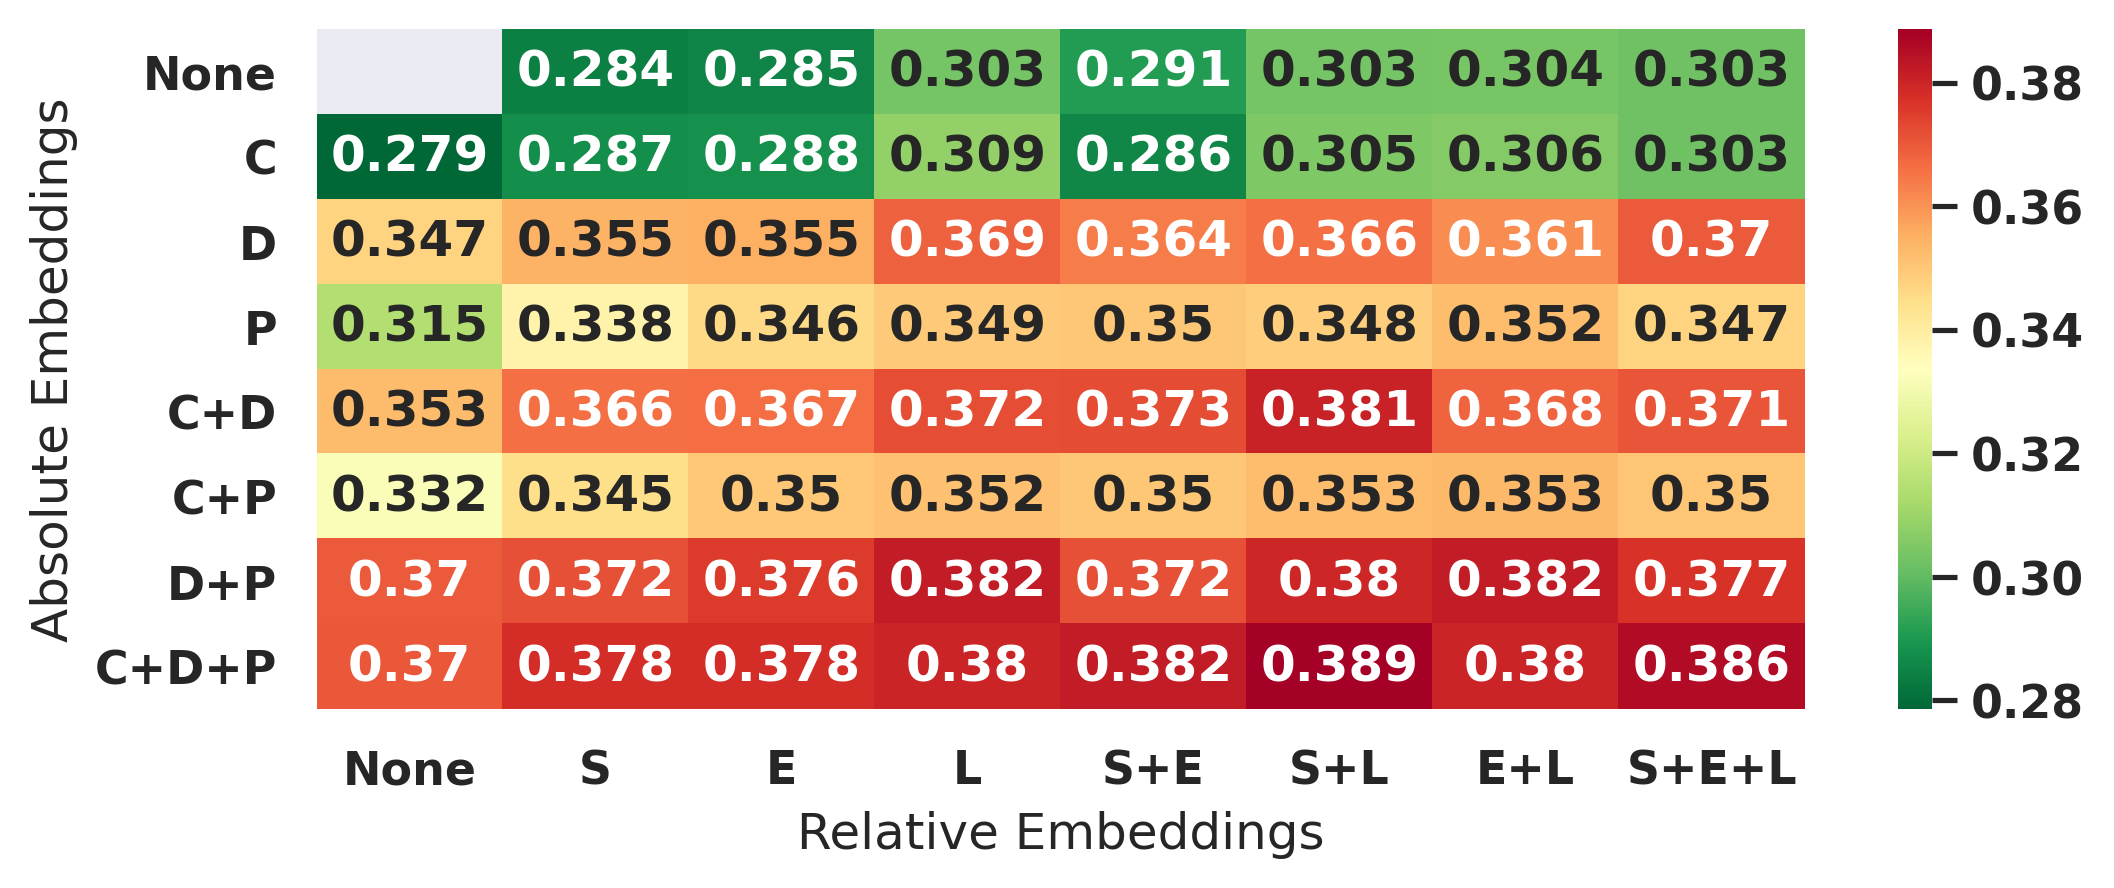
\includegraphics[width=\linewidth]{figures/combinations/game_60.png}
    %\caption{Amazon Game}
  \end{minipage}
  \caption{NDCG@10 Comparison with All Possible Combinations of Positional Embeddings on ML-1M (left) and Game (right) Dataset. C, D, P, S, E and L represent \textbf{Con}, \textbf{Day}, \textbf{Pos}, \textbf{Sin}, \textbf{Exp} and \textbf{Log}, repectively. We used $h=60$ for all experiments.}
  \Description[The figure describes heatmaps of NDCG@10 comparison with all possible combinations of embedding types on MovieLens 1M and Amazon Game]{The left figure is a heatmap of NDCG@10 comparison with all possible combinations of embedding types on MovieLens 1M. Absolute embeddings lie on y-axis and relative embeddings lie on x-axis. As we move further into the x-axis, the heatmap gets hotter. Columns with Log embedding seems to be the hottest. The right figure describes the same heatmap on Amazon Game. As we move further down on y-axis, the heatmap gets hotter. Rows with Day embedding seems to be the hottest.}
  \label{fig:tesearch}
\end{figure*}
Figure \ref{fig:tesearch} shows the comparison of all possible combinations of temporal embeddings on ML-1M and Amazon Game dataset. We fixed all other hyperparameters (e.g., $h=60$). Interestingly, the importance of each embedding seems to differ in each dataset. In ML-1M, relative position embeddings (especially \textbf{Log}) seem to play an important role, whereas in Amazon Game, absolute position embeddings (especially \textbf{Day}) seem to be essential. Therefore, the optimal combination is also different for each dataset. Further analysis with different $h$ shows us that while optimal combination differs slightly for each $h$, the overall tendency stays the same for each dataset. The same applies to other datasets. This suggests that datasets with distinct characteristics require carefully chosen temporal embeddings that provide the right views on the context of user-item interactions. Note that while we only used $n=2\text{ and }4$ for Table \ref{tab:results} to be fair with other baselines, using all possible $n$ can further improve our performance.
% EH: 아래와 같은 문장 정도면 어떨까 
%When we apply the same analysis on the different datasets, the best joint set of embeddings is different. According to our observation, each dataset has unique contextual characteristics which is useful information to predict the next behavior. 
%This suggests that datasets with different characteristics require different view on the positions of user-item interactions in a sequence. [ANALYZE WHY]

% In this section we seek to study the effect of various positional embeddings. To assess the contribution of each positional embedding type in more detail, we ran an extensive experiment to test all combinations of positional embeddings. Figure-\ref{fig:tesearch} shows the comparison of NDCG@10 performance on ML-1M and Amazon Game dataset. All other hyperparameters were kept equal.

% \begin{figure}[ht]
  \centering
  \begin{subfigure}[ht]{.49\linewidth}
    \centering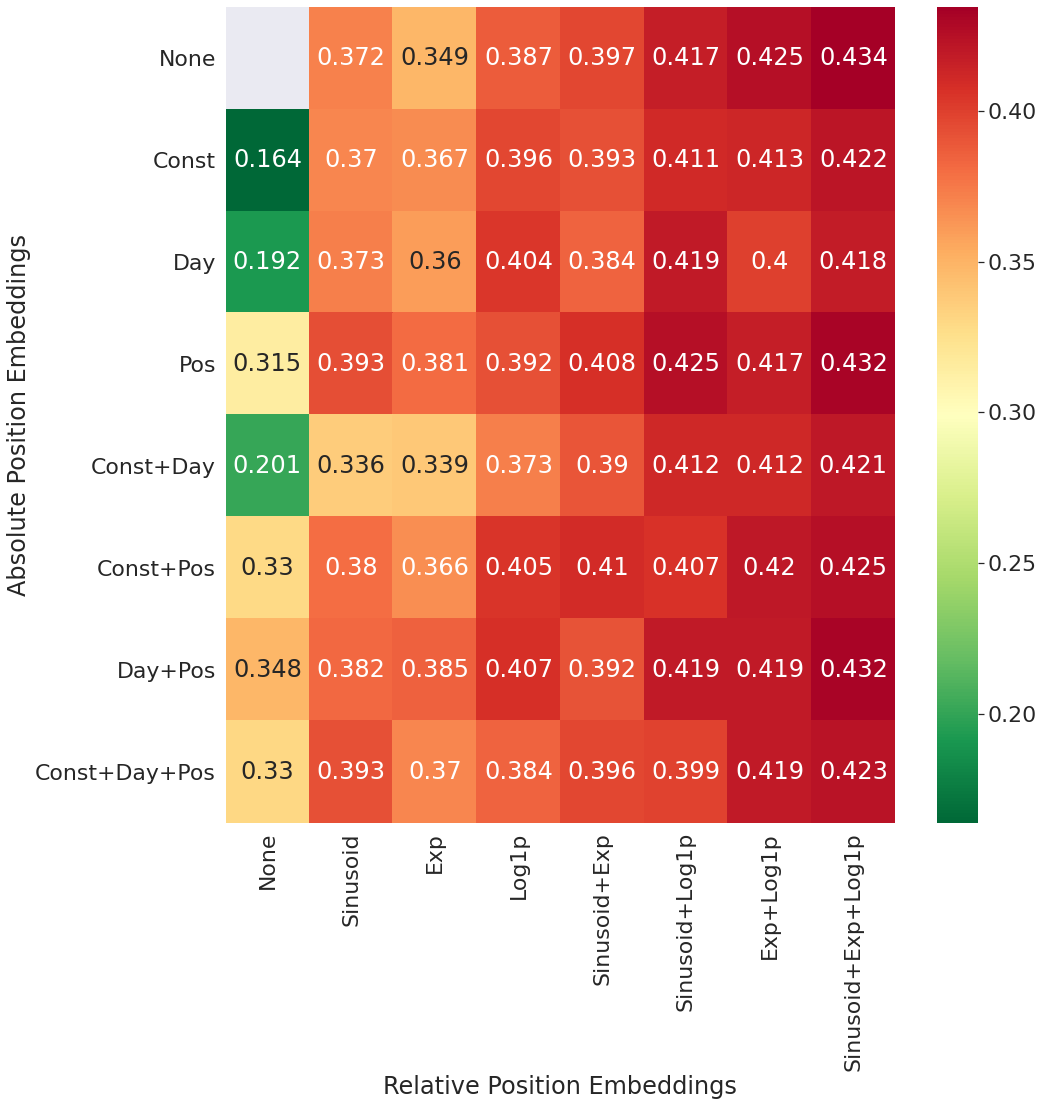
\includegraphics[width=.95\linewidth]{figures/tesearch.png}
    \caption{MovieLens 1M}
  \end{subfigure}
  \begin{subfigure}[ht]{.49\linewidth}
    \centering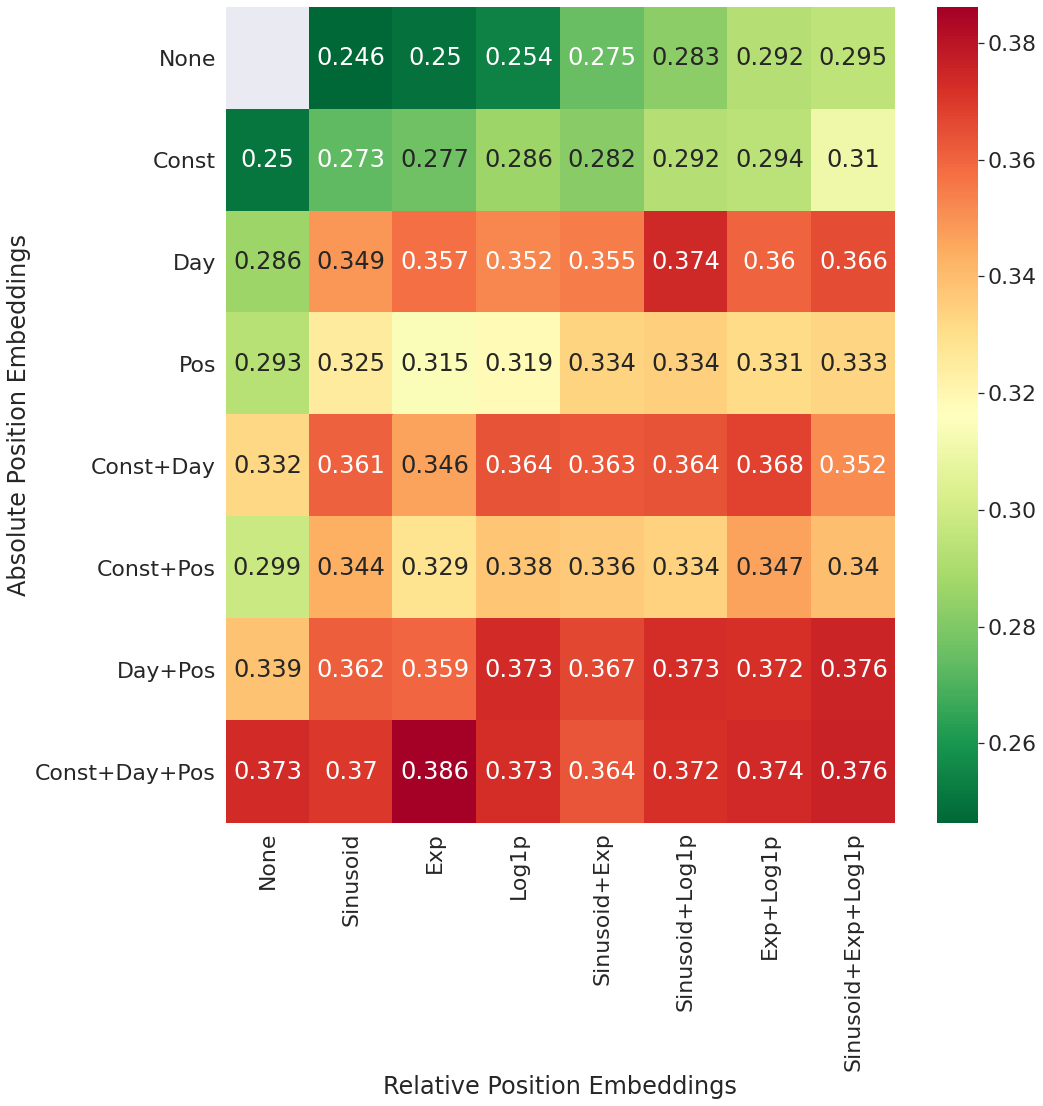
\includegraphics[width=.95\linewidth]{figures/tesearch_game.png}
    \caption{Amazon Game}
  \end{subfigure}
  \caption{NDCG@10 Comparison with All Possible Combinations of Positional Embeddings on ML-1M and Game Dataset}
  \Description{TODO:Description}
  \label{fig:tesearch}
\end{figure}

% Interestingly, the importance of each embedding seems to differ in each dataset. In ML-1M, relative position embeddings(especially \textbf{Log1p}) seem to play an important role, whereas in Amazon Game, absolute position embeddings(especially \textbf{Pos} and \textbf{Day}) seem to be essential. In ML-1M, the optimal performance is achieved when we use all three relative position embeddings and none of the absolute position embeddings. In contrast, using all three absolute position embeddings with only \textbf{Exp} relative embedding works best in Amazon Game. This proves that datasets with different characteristics require different view on the positions of user-item interactions in a sequence.

% %\begin{figure}[ht]
  \centering
  
  \begin{subfigure}[ht]{.33\linewidth}
    \centering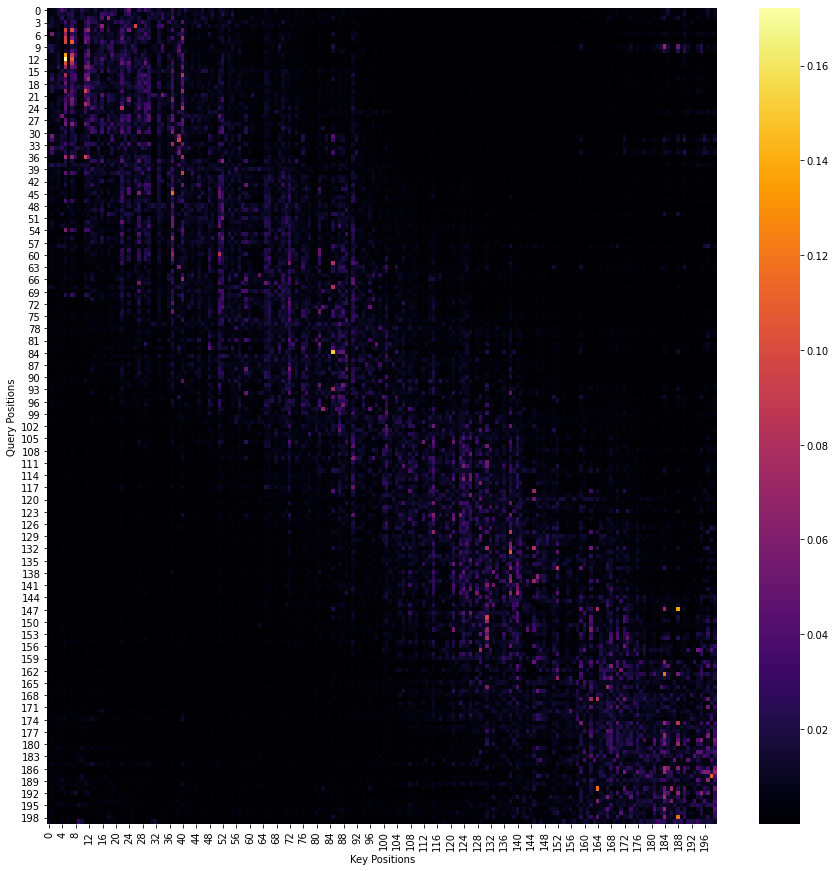
\includegraphics[width=.95\linewidth]{figures/attn1/L0BPH1.png}
    \caption{\textbf{Pos} Layer 0 Head 1}
  \end{subfigure}
  \begin{subfigure}[ht]{.33\linewidth}
    \centering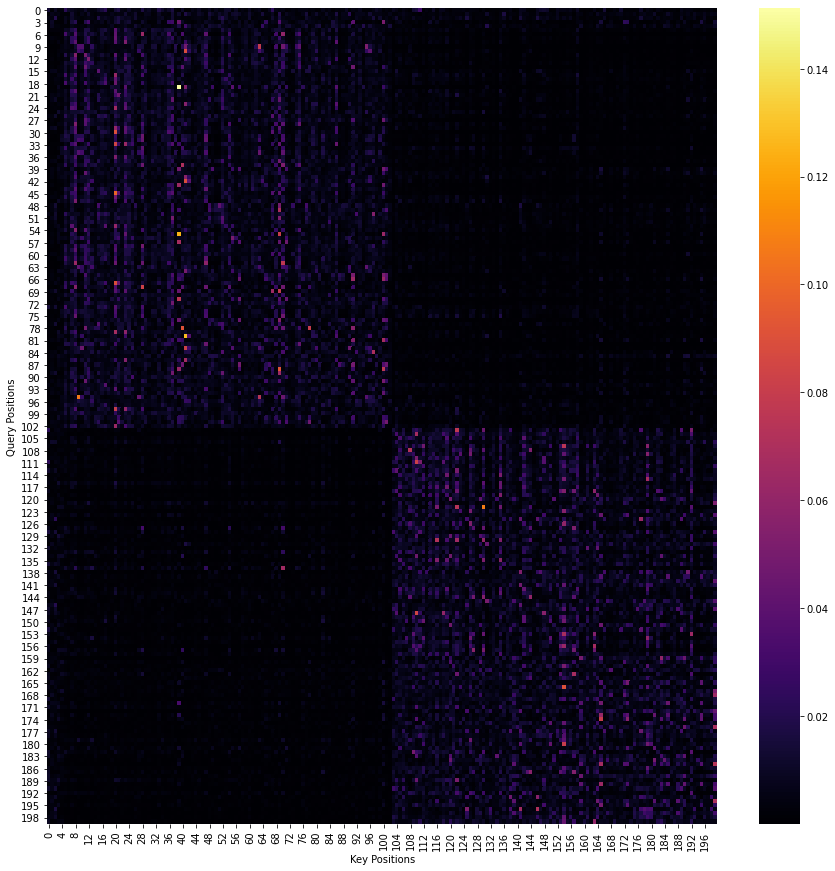
\includegraphics[width=.95\linewidth]{figures/attn1/L0BDH0.png}
    \caption{\textbf{Day} Layer 0 Head 0}
  \end{subfigure}
  \begin{subfigure}[ht]{.33\linewidth}
    \centering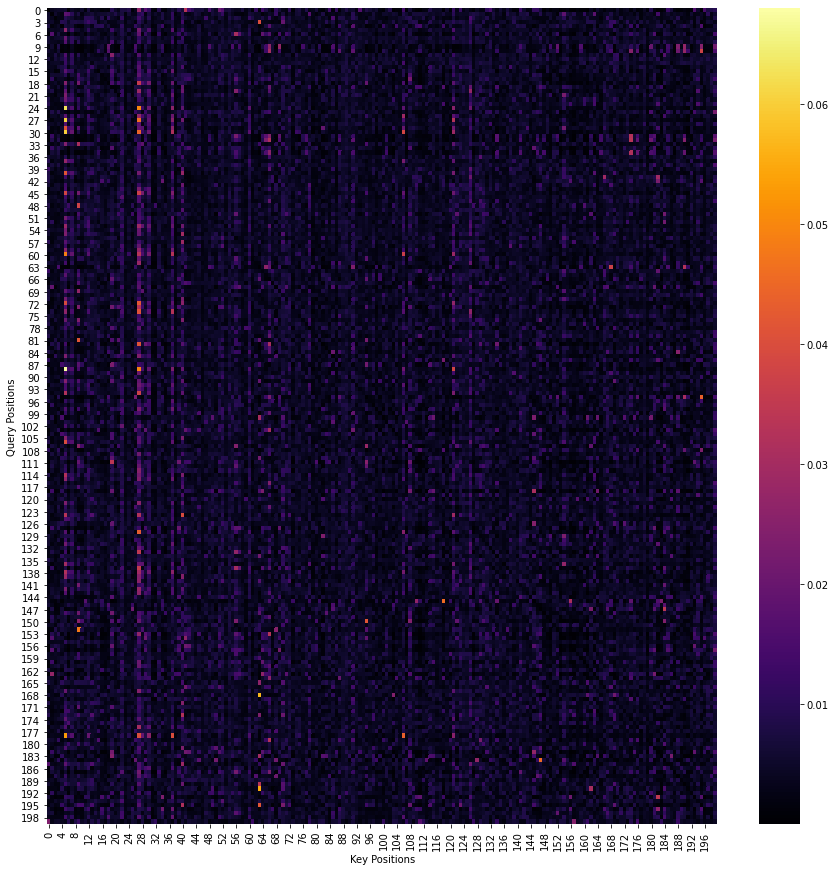
\includegraphics[width=.95\linewidth]{figures/attn1/L0BCH0.png}
    \caption{\textbf{Const} Layer 0 Head 0}
  \end{subfigure}
  \begin{subfigure}[ht]{.33\linewidth}
    \centering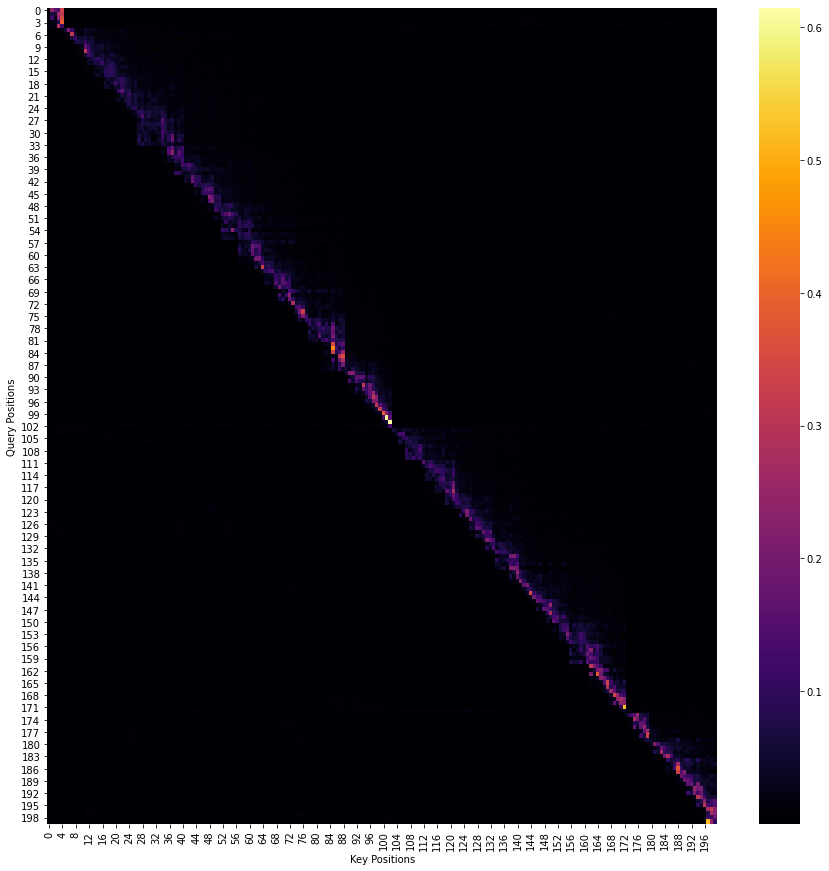
\includegraphics[width=.95\linewidth]{figures/attn1/L0BSH0.png}
    \caption{\textbf{Sinusoid} Layer 0 Head 0}
  \end{subfigure}
  \begin{subfigure}[ht]{.33\linewidth}
    \centering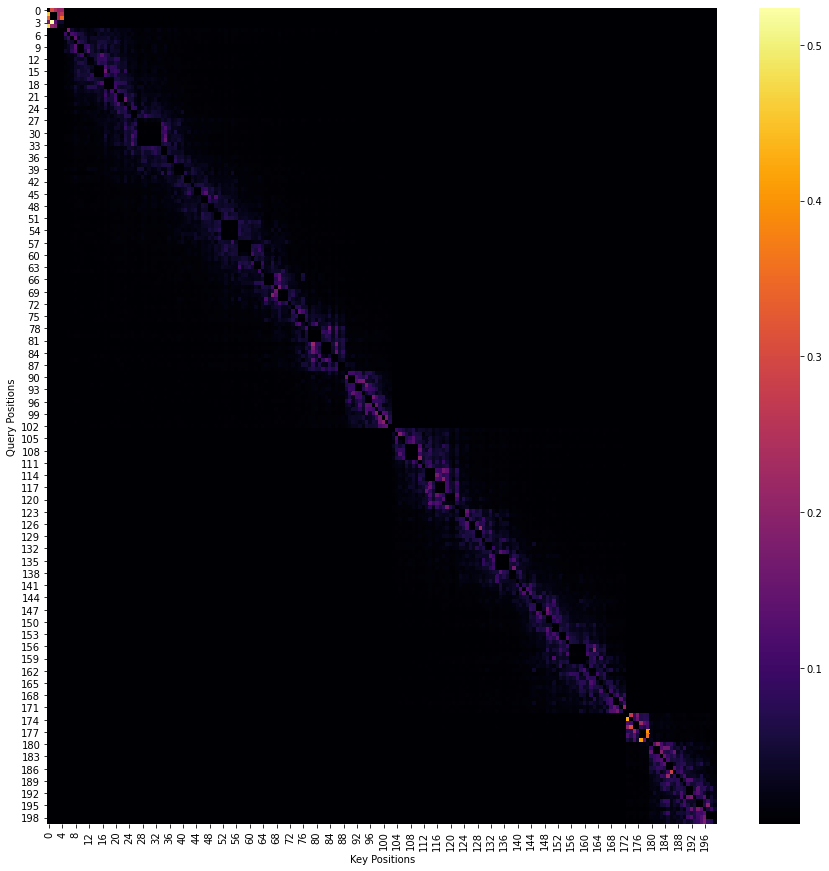
\includegraphics[width=.95\linewidth]{figures/attn1/L0BEH0.png}
    \caption{\textbf{Exp} Layer 0 Head 0}
  \end{subfigure}
  \begin{subfigure}[ht]{.33\linewidth}
    \centering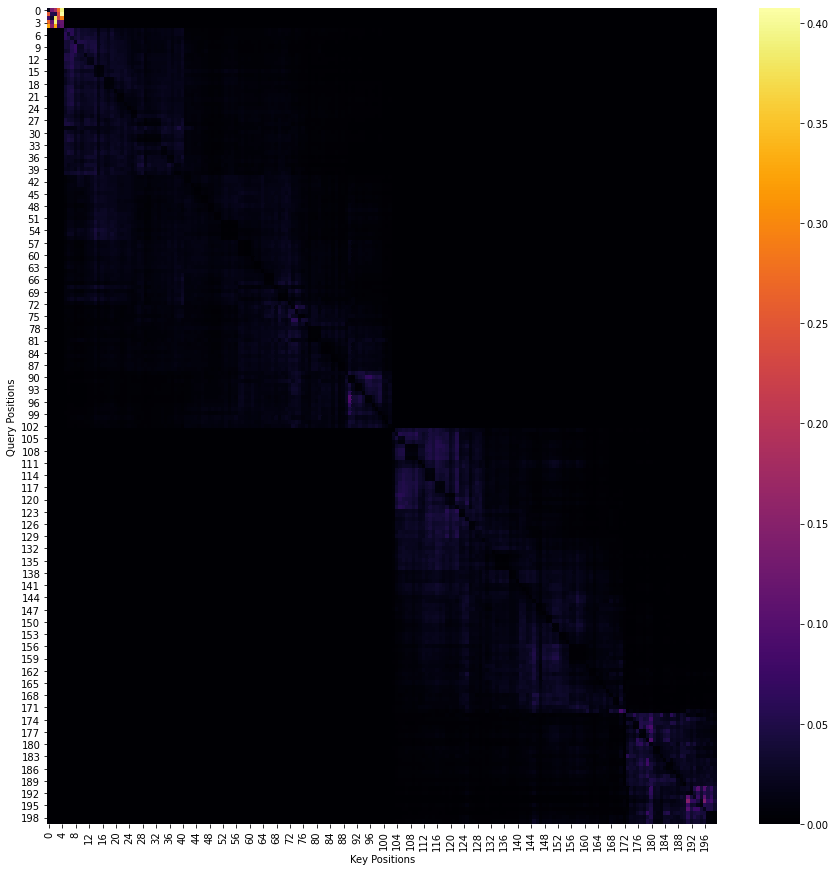
\includegraphics[width=.95\linewidth]{figures/attn1/L1BLH0.png}
    \caption{\textbf{Log1p} Layer 1 Head 0}
  \end{subfigure}
  
  %\subfigure{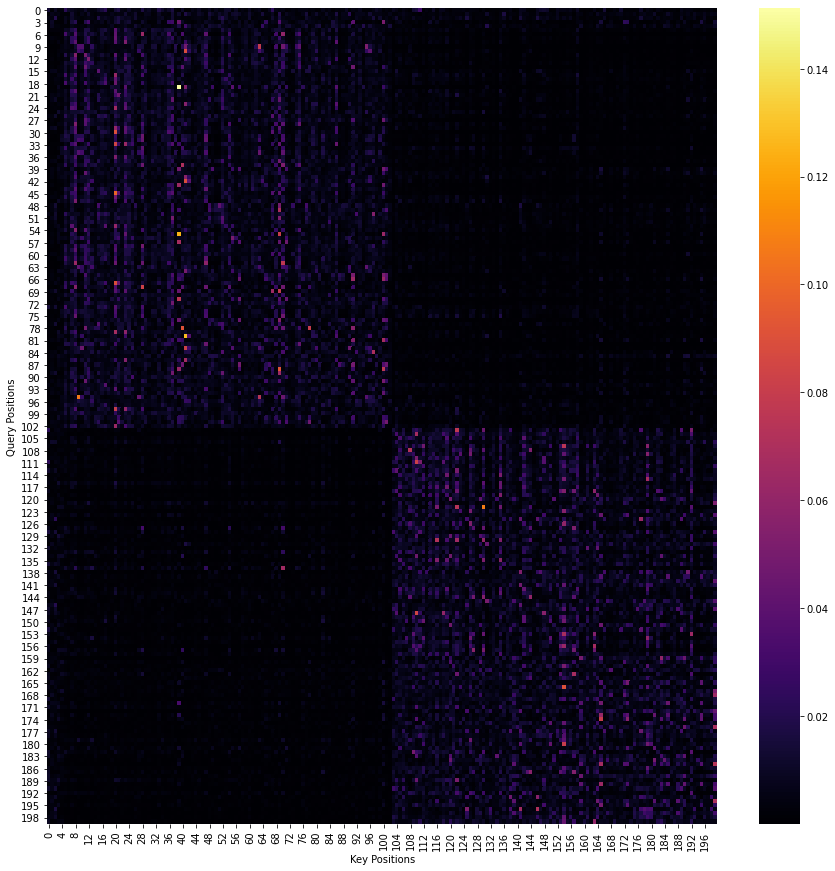
\includegraphics[width=0.5\linewidth]{figures/attn1/L0BDH0.png}}
  %\subfigure{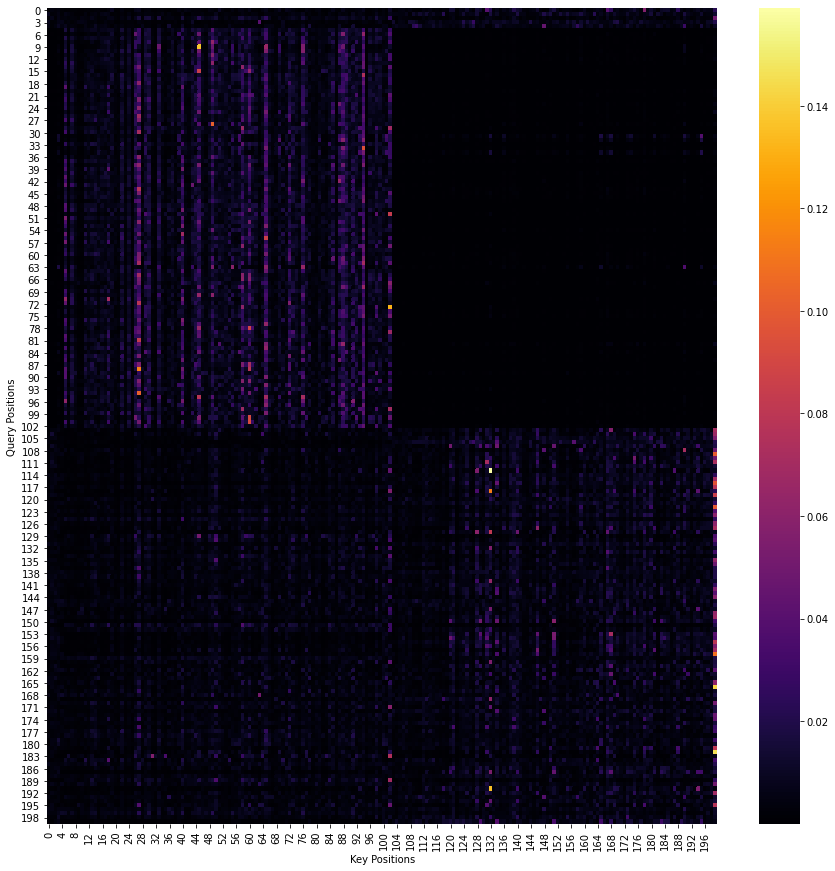
\includegraphics[width=0.5\linewidth]{figures/attn1/L0BDH1.png}}
  \caption{Attention Score Maps (Might need to change the figures to ones with shorter sequences (so that they are more clear))}
  \Description{TODO:Description}
  \label{fig:attnmaps}
\end{figure}

% \begin{table}[ht]
\caption{Gradient Comparison for Each Embedding Type}
\label{tab:grad_cam}
\begin{tabular}{@{}lllllll@{}}
\toprule
{Dataset} & {Pos}           & {Day}              & {Const}            & {Sinusoid}         & {Exp}           & {Log1p}         \\ \midrule
{ML1M}    & {4.79\%}        & {5.34\%}           & {1.50\%}           & {\textbf{51.34\%}} & {7.08\%}        & {\underline{29.94\%}} \\
{ML20M}   & {\underline{19.60\%}} & {5.50\%}           & {6.11\%}           & {\textbf{24.51\%}} & {\underline{22.58\%}} & {\underline{21.70\%}} \\
{Beauty}  & {1.03\%}        & {8.39\%}           & {\textbf{57.12\%}} & {9.79\%}           & {0.69\%}        & {\underline{22.98\%}} \\
{Game}    & {\underline{40.39\%}} & {\textbf{49.57\%}} & {1.96\%}           & {1.19\%}           & {1.37\%}        & {5.51\%}  \\ \bottomrule
\end{tabular}
\end{table}

% To further measure the contributions of each embedding type, we applied a method similar to Grad-CAM\cite{GRADCAM} to our fully equipped model(with all 6 embedding types). For every sequence in the test data, we took the output from the final layer of our self-attention block stacks $\mathbf{Z}^L = [\mathbf{Z}^L_1, ..., \mathbf{Z}^L_\Sigma]$, and then computed the gradient of each output with regard to the answer item's logit $y^c$:
% \begin{equation}
%     g_i = \frac{dy^c}{dZ^L_i}
% \end{equation}
% Similar to \cite{GRADCAM}, we only took positive gradients from $g_i$ to measure their positive influence on the answer's logit. We calculated the average of their sums and then applied softmax to get Table-\ref{tab:grad_cam}.

% As we expected, relative position embeddings were dominant in MovieLens datasets, while absolute position embeddings were dominant in Amazon datasets. Moreover, as we saw in Figure-\ref{fig:tesearch}-(b), \textbf{Pos} and \textbf{Day} play very important roles in Amazon Game. Unlike Figure-\ref{fig:tesearch}-(a), \textbf{Sinusoid} seems to be more influential than \textbf{Log1p} in ML-1M. However, it is interesting to note that \textbf{Log1p} stays somewhat influential throughout all datasets. Another interesting observation is the dominance of \textbf{Const} in Amazon Beauty. This seems to suggest that positional bias is relatively less important in Amazon Beauty dataset. These results show that one must carefully design the positional embeddings in the recommendation system by considering the characteristics of the dataset.

% %Due to limited space, we study the images of attention score maps for each embedding type in Appendix-\ref{app:attnmaps}.

% %Figure-\ref{fig:attnmaps} shows the attention score maps for different positional embeddings. Due to limited space, we only present representative maps. We provide full-scope attention maps in Appendix-

% %(Analysis on Figure-\ref{fig:attnmaps})


%\subsection{Effect of Multi Self-attention Blocks}
%Although we let all transformer-based models have the same number of layers and heads in our experiments, MEANTIME has more parameters than SASRec, TiSASRec, and BERT4Rec since it employs 6 self-attention blocks per layer in contrast to 1. This might seem unfair since the performance gain could have come from the larger parameter size, or from the multi-path self-attention. To prove that this is not the case, we also experimented with the adjusted baseline models where they also have 6 self-attention blocks per layer. We call them \textbf{buffed} models. 

\begin{table}[h]
\caption{Performance Comparison with Buffed Baselines.}
\label{tab:buff_results}
\begin{tabular}{@{}lrrrrr@{}}
\toprule
{Metrics} & {SASRec-Buffed}& {TiSASRec-Buffed} & {BERT4Rec-Buffed} & {MEANTIME}      \\ \midrule
{Recall@5}  & {0.5512} & {0.5528} & {0.5916} & {\textbf{0.6154}} \\
{Recall@10}  & {0.6853} & {0.6856} & {0.6987} & {\textbf{0.7268}} \\
{NDCG@5}   & {0.3955} & {0.3962}  & {0.4437} & {\textbf{0.4690}} \\
{NDCG@10}  & {0.4390} & {0.4393}  & {0.4785} & {\textbf{0.5052}} \\ \bottomrule
\end{tabular}
\end{table}

Table-\ref{tab:buff_results} shows the comparison results. All experiments were done with ML-1M dataset, hidden dimension size $h=64$, dropout ratio 0.2 and weight decay 0. The result clearly shows that the strong performance of MEANTIME does not merely come from large parameter size nor multi-path self-attention.

%\subsection{Effect of Information Separation}

%\subsection{Effect of Hidden Dimension Size}
%Here we study the effect of hidden dimension size on each dataset. We experiment with $h \in \{16, 32, 64, 128\}$ while keeping other hyperpameters the same.

\begin{figure}[ht]
  \centering
  
  \begin{subfigure}[ht]{\linewidth}
    \centering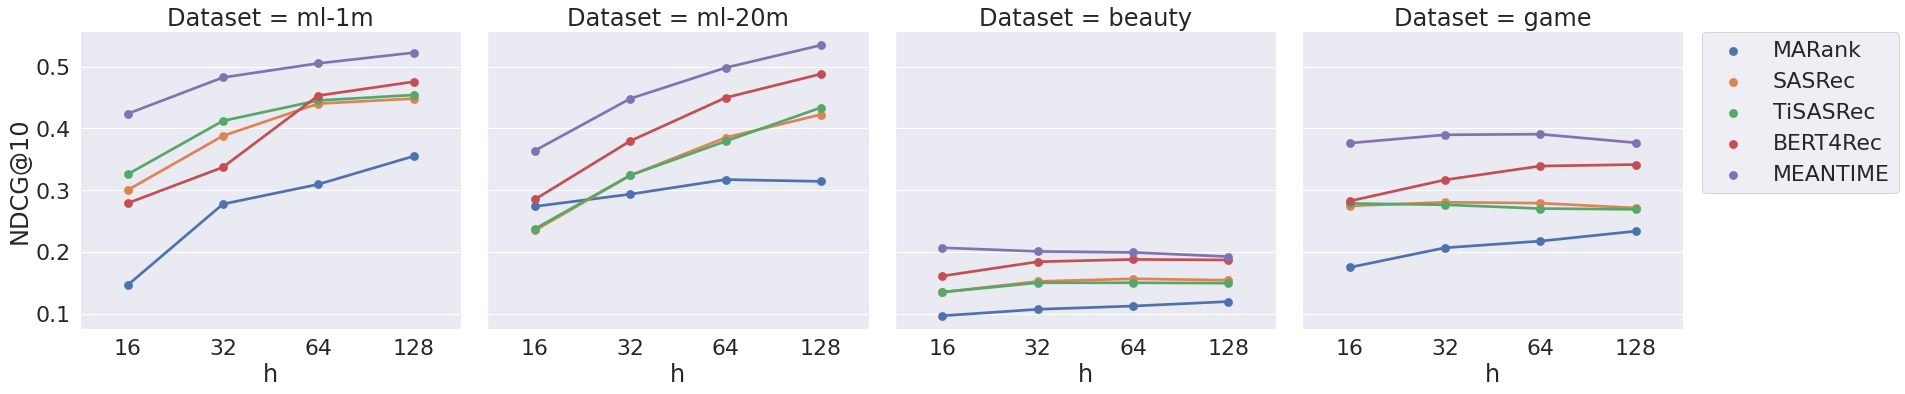
\includegraphics[width=\linewidth]{figures/impact_h/n10.png}
    \caption{NDCG@10}
  \end{subfigure}
  \begin{subfigure}[ht]{\linewidth}
    \centering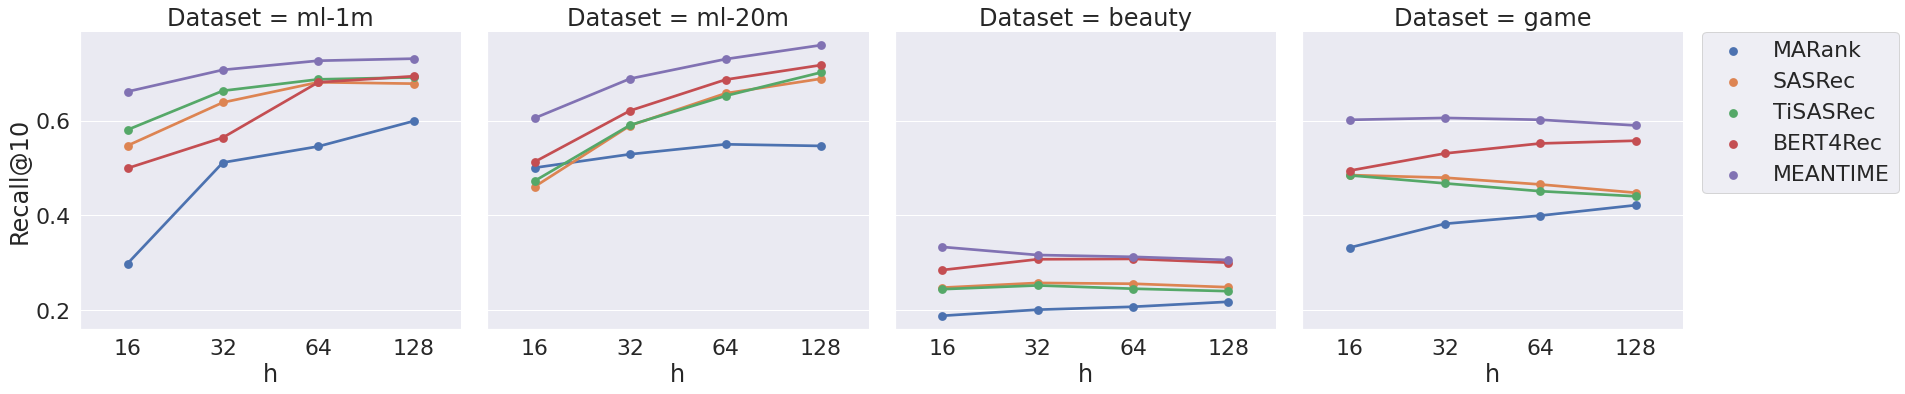
\includegraphics[width=\linewidth]{figures/impact_h/r10.png}
    \caption{Recall@10}
  \end{subfigure}
  
  \caption{Effect of hidden dimension size on NDCG@10 and Recall@10}
  \Description{TODO:Description}
  \label{fig:himpact}
\end{figure}

Figure-\ref{fig:himpact} shows the comparison results. We observe that optimal hidden dimension size differs between datasets. Interestingly, MEANTIME works optimally at $h = 16$ in Amazon Beauty dataset. This is probably because it is the most sparse dataset of the four, which makes it prone to overfitting.

We also observe that without extensive hyperparameter tuning, TiSASRec\cite{TISASRec}, which uses temporal infromation to improve SASRec\cite{SASRec}, sometimes doesn't outperform SASRec. In contrast, MEANTIME, which improves BERT4Rec\cite{BERT4Rec} with temporal information, always outperforms BERT4Rec (and all other baseline models) even without parameter tuning. This seems to prove the superiority of our model. [TOO MUCH BRAGGING?]

%\subsection{Effect of freq \& $\tau$}
%\begin{figure}[ht]
  \centering
  \begin{subfigure}[ht]{.45\linewidth}
    \centering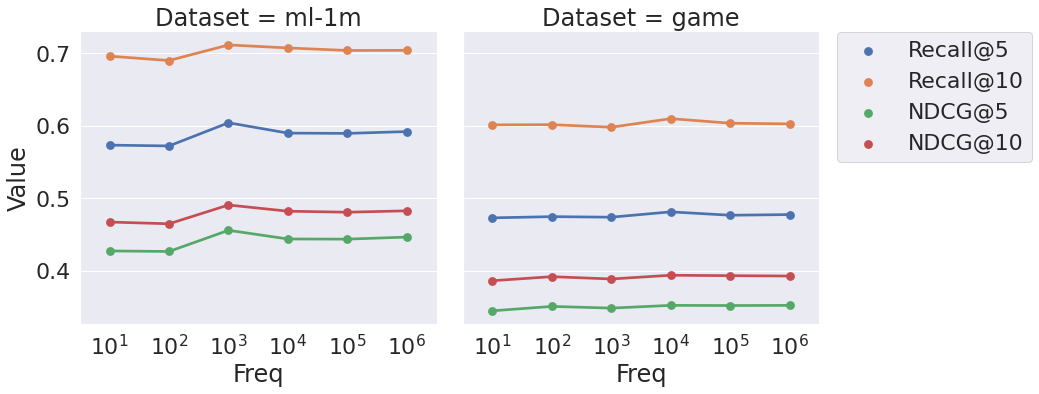
\includegraphics[width=\linewidth]{figures/freq_tau/freq_search.png}
    \caption{Effect of \textit{freq}}
  \end{subfigure}
  \begin{subfigure}[ht]{.45\linewidth}
    \centering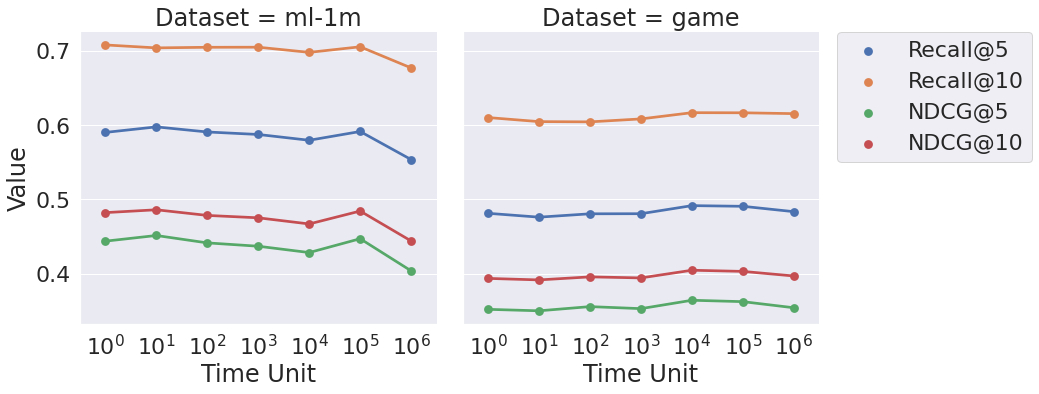
\includegraphics[width=\linewidth]{figures/freq_tau/tau_search.png}
    \caption{Effect of $\tau$}
  \end{subfigure}
  \caption{Effect of \textit{freq} and $\tau$ on performance}
  \Description{TODO:Description}
  \label{fig:freq_tau}
\end{figure}